% Figure 1 (a): the fork probe as a pipeline. Images: exact replays of held-out state ep63_seed104_s74
% (paper/render_fork_frames.py). Ghost images average the 64 imagined starts / endings.
\begin{tikzpicture}[
  font=\footnotesize, every node/.append style={execute at begin node={\hyphenpenalty=10000\relax}},
  stage/.style={font=\scriptsize\bfseries\color{inkc}, anchor=south},
  note/.style={font=\scriptsize, text=mutedc, align=center, anchor=north, text width=2.3cm},
  img/.style={inner sep=0pt, draw=linec, line width=0.4pt},
  card/.style={draw=linec, fill=cardc, rounded corners=3pt, line width=0.4pt, align=center,
               minimum height=2.15cm, inner sep=3pt, font=\scriptsize},
  flow/.style={-{Stealth[length=4pt]}, line width=0.7pt, draw=mutedc},
]
\def\w{2.15cm}
% 1 camera image
\node[img] (cam) at (0,0) {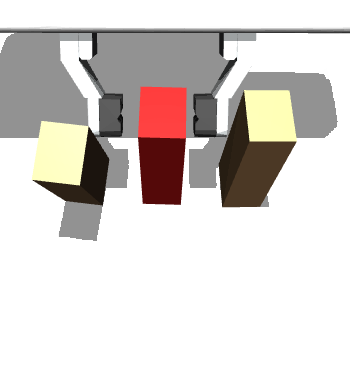
\includegraphics[width=\w]{fig_assets/crop_start.png}};
\node[stage] at (cam.north) {camera image};
\node[font=\small\bfseries, anchor=south east] at ([xshift=-2pt,yshift=10pt]cam.north west) {(a)};
\node[note] at (cam.south) {perceived block poses\\(2.5\,mm error)};
% 2 the robot's uncertainty
\node[img, right=0.55cm of cam] (unc) {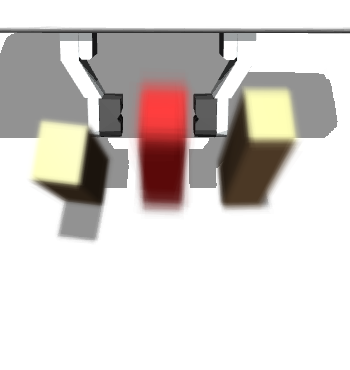
\includegraphics[width=\w]{fig_assets/crop_start_ghost.png}};
\node[stage] at (unc.north) {\textcolor{tealc}{its own uncertainty}};
\node[note] at (unc.south) {64 plausible scenes (measured perception error) $\times$ measured execution error};
% 3 rollout engine
\node[card, right=0.55cm of unc, text width=2.15cm] (eng) {%
  \textbf{rollout engine}\\[3pt]
  8-step chunk\\then 30-step\\imagined hold\\[4pt]
  \textcolor{inkc}{MuJoCo}\\{\color{mutedc}(reference)}\\[1pt] or\\[1pt]
  \textcolor{violetc}{learned world model}};
% 4 imagined futures
\node[img, right=0.55cm of eng] (fut) {
\includegraphics[width=\w]{fig_assets/crop_end_ghost.png}};
\node[stage] at (fut.north) {\textcolor{orangec}{64 imagined futures}};
\node[note] at (fut.south) {the neighbour stays (31)\\or topples (33)};
% 5 decision
\node[card, right=0.55cm of fut, text width=1.9cm] (dec) {%
  \textbf{split test}\\[3pt]
  two persistent,\\well-separated\\groups?\\[4pt]
  \textcolor{orangec}{\textbf{yes: fragile}}\\[1pt]
  {\color{mutedc}slow down,\\re-perceive, replan}};
\draw[flow] (cam.east) -- (unc.west);
\draw[flow] (unc.east) -- (eng.west);
\draw[flow] (eng.east) -- (fut.west);
\draw[flow] (fut.east) -- (dec.west);
\end{tikzpicture}
